\documentclass{article}
\usepackage{amsfonts, amsthm, amsmath}

\usepackage{geometry, graphicx}
\usepackage{algorithm, algorithmic}
\usepackage{bm}
\geometry{left = 5em, right = 5em}

\def\showtopic{Mathematical Image Processing Homework 2}
\def\showtitle{PDE Methods for Image Restoration}
\def\showabs{PDE based Model}
\def\showauthor{Yuanfeng Shi, 1800010697}

\title{\showtitle}
\author{\showauthor}

\usepackage{fancyhdr}  
\pagestyle{fancy}
\lhead{\textbf {\showtopic} }
\chead{} 
\rhead{\textbf {\showabs} }
\lfoot{} 
\cfoot{\thepage}
\rfoot{} 
\renewcommand{\headrulewidth}{0.4pt} 


\usepackage{listings}
\lstset{language=Matlab}
\lstset{breaklines}
\lstset{extendedchars=false}
\newtheorem{proposition}{Proposition}
\newtheorem{remark}{Remark}
\begin{document}
\maketitle
\thispagestyle{fancy}
\section{Introduction}
     PDE based models have a uniform form in general case:
\begin{equation}
\frac{\partial u}{\partial t} + F(x,u(t,x), \nabla u(t,x), \nabla^2 u(t,x)) = 0
\end{equation}
with the initial boundary value condition $u(0,x) = f(x)$, where the $f$ is the observed image. Here the $\nabla$ and $\nabla^2$ is the gradient and the Hessian matrix of the given function $u$. 

What these PDE models for image restoration have in common is that they seek a good balance
between the two seemingly contradictory objectives: smoothness at locations where
noise or other artefacts have been removed, and preservation or even enhancement of
the sharpness of edges, corners, etc.

The choice of $F$ should consider two aspects: The first part is that the solution $u$ is a smoothed result of $f$ in order to remove the Gaussian white noise; The second part is preserving edges, textures and other information. This seems a contradiction between smoothing and enhancing, so we need to make a trade-off between the two properties. 

The report is organized as three parts: The first part is about the smoothing operator: heat diffusion. The second term is about the smoothing--enhancing operator: Perona--Malik diffusion and the last is about enhancing operator: Rudin--Osher shock filter. For each part, we will introduce the definition, properties, the algorithm, and the numerical performance. 

\section{Heat Diffusion}
\subsection{Definition}
The heat equation is defined on the whole $\mathbb R^2$:
\begin{equation}
u_t = \triangle u ,~~~~~ u(0,\cdot) = f
\end{equation}
It is easy to check once the initial function $f$ is locally $L^1$, the solution will be $C^\infty$ functions for all positive $t$, as we can write the solution as a convolution:
\begin{equation}
u(t,\cdot) = G_{\sqrt{2t}} * f,
\end{equation}
where $G_{\sigma}$ is the gaussian distribution with zero mean and $\sigma^2$ variance, i.e. $$G_\sigma = \frac{1}{2\pi\sigma}exp(-\frac{x^2}{2\sigma^2}).$$

\subsection{Properties}
Since the Laplacian operator is isotropic, if we use the orthogonal system $\{N = \nabla u / |
\nabla u| T\}$ we will get $\triangle u = u_{NN} + u_{TT}$. This means the heat kernel will smooth the normal direction as well as the tangent direction.

Also, the heat diffusion has some properties desired in the image science:
\begin{enumerate}
\item Gray-level shift invariance
\item Translation invariance
\item Scale invariance 
\item Isometry invariance
\item Conservation of average value
\item Semigroup property
\item Comparison principle
\end{enumerate}

However, the drawback is obvious: it is too smoothing and edges will be lost in a few time.

\subsection{Algorithm}
The algorithm of heat diffusion is 
$$u^0 = f$$
$$u^{(n+1)} = u^{n} + \Delta t~\triangle u^n.$$
Here the $\Delta$ is the discrete laplacian operator i.e.
$$\triangle u_{i,j} = \frac{u_{i,j+1} + u_{i,j-1} + u_{i+1,j} + u_{i-1,j} - 4u_{i,j}}{4}.$$

\begin{algorithm}
\caption{$u = heat(f,T,\Delta t)$}
\begin{algorithmic}[1]
\STATE $u =f$
\FOR {$i = 1:T$}
\STATE Compute the Laplacian of $u=:L$
\STATE $u = u + \Delta t * L$
\ENDFOR
\end{algorithmic}
\end{algorithm}
In practical, we can use a convolution to implement the subroutine.

\subsection{Numerical Result}
The numerical result uses the `circular' boundary condition when operating the Laplacian. And we always take $\Delta t = 0.01$, noise = $0.05 * randn(n,n)$.

We notice that besides removing the noise, the heat diffusion makes the image more blurred. When the iteration time (aka evolution time) is larger, the long time behaviour will be worse and worse. We choose the classical image 'peppers256' and 'barbara' and evolving them at various time step $T$ to show what happens when the evolution time gets larger.

\begin{figure}[H]
\label{fig:heat-l-c}
\begin{center}
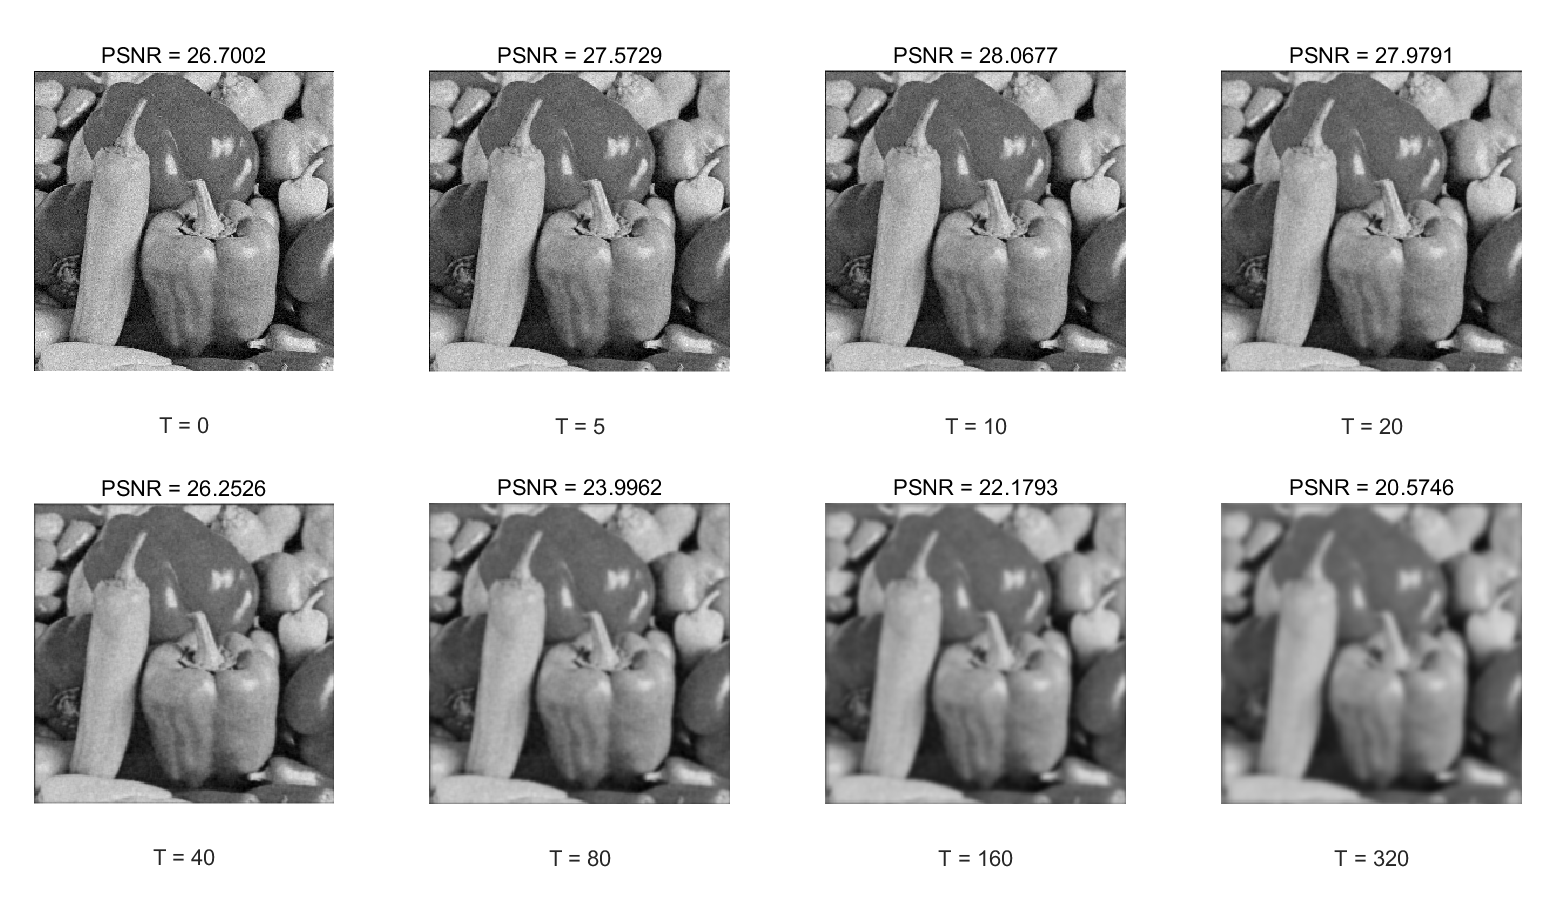
\includegraphics[scale=.38]{1.png}

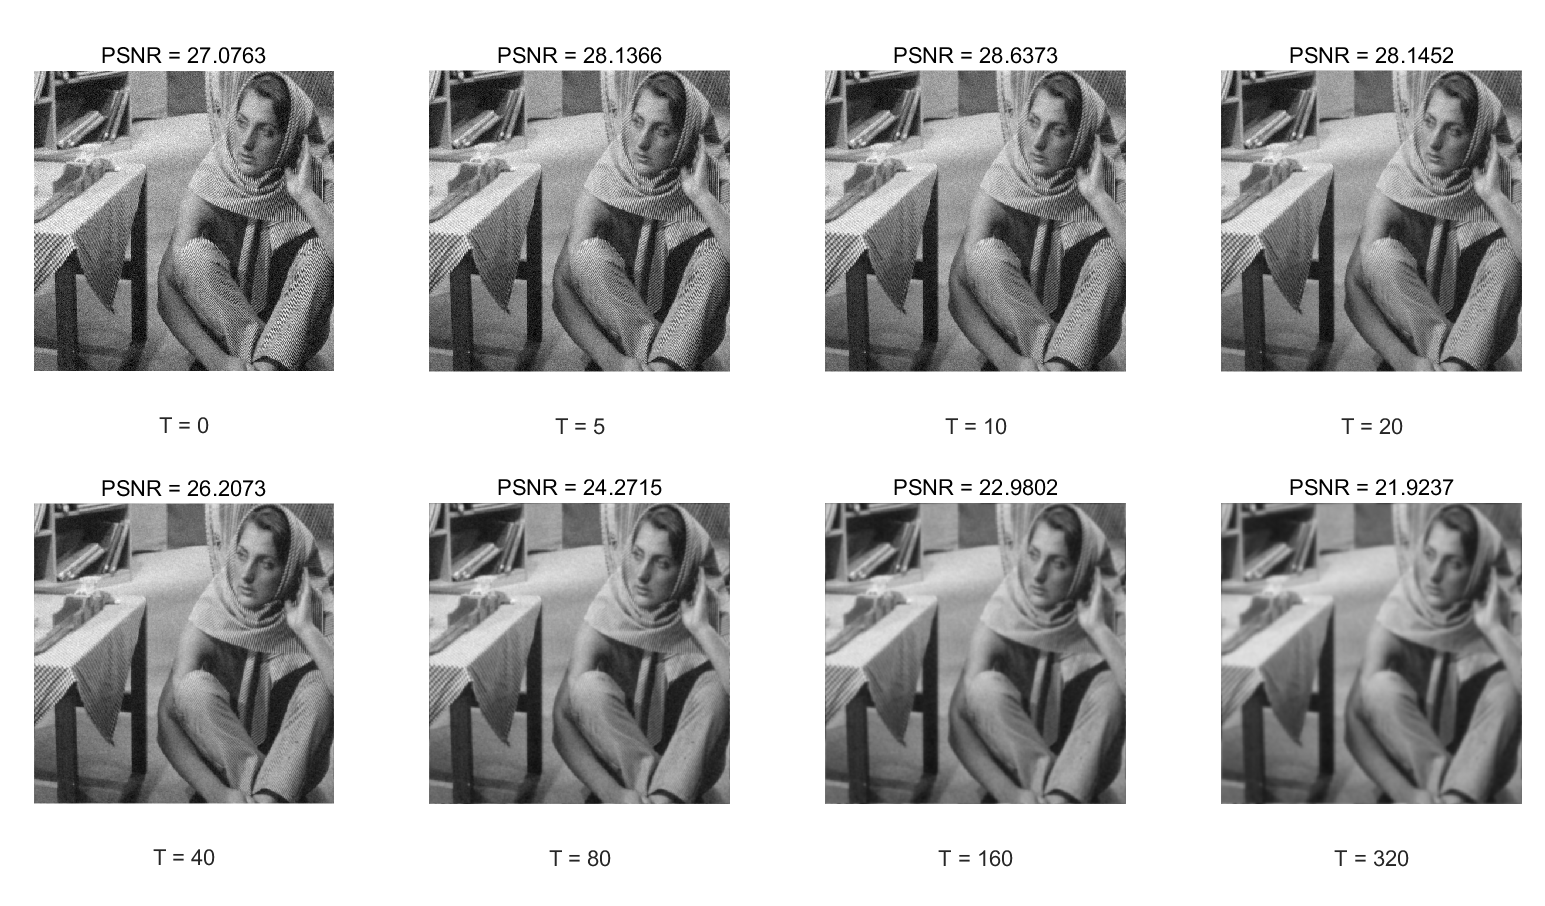
\includegraphics[scale=.38]{2.png}
\end{center}
\caption{The long time behaviour of heat diffusion: noise = 0.05 * randn(n,n). $\Delta t = 0.01$. Notice when the time tends to the infinity, the image will become constant.} 
\end{figure}

\section{Perona and Malik Nonlinear Diffusion}

\subsection{Algorithm}
The main subroutine of Perona--Malik diffusion is analogous to the Heat diffusion, and the direction derivative will also be computed by convoution. However, when discrtizing the gradient, we will split two direction and consider them respectively. 

Consider the formulation:
$$u^{n+1} = u^{n} + \Delta t~\sum c(|\delta_i u|^2)~\delta_i u.$$
Here $\delta_i u$ is one of the four cases:
$$\delta_x^+ u_{i,j} = u_{i+1,j}-u_{i,j}$$
$$\delta_y^+ u_{i,j} = u_{i,j+1}-u_{i,j}$$
$$\delta_x^- u_{i,j} = u_{i,j}-u_{i-1,j}$$
$$\delta_y^- u_{i,j} = u_{i,j}-u_{i,j-1}$$.
And $c()$ will be chosen as $$c(s) = \frac{1}{1+s/K}$$

\begin{algorithm}
\caption{$u = perona\_malik(f,T,\Delta t,c)$}
\begin{algorithmic}[1]
\STATE $u=f$
\FOR{$i=0:T$}
\FOR {each direction $dir$}
\STATE Compute the direction partial difference of image $u$ as $u_{dir}$.
\ENDFOR
\STATE $u^{n+1} = u^{n} + \Delta t~\sum_{dir}c(|u_{dir}|^2)~u_{dir}.$
\ENDFOR
\end{algorithmic}
\end{algorithm}

\subsection{Numerical Result}
In this section we show the the long time behaviour of Perona--Malik algorithm. The crucial observation is that when it will be more robust than the heat diffusion during a long time: the restoration quality when decreases slowly than the heat diffusion performs.
\begin{figure}[H]
\begin{center}
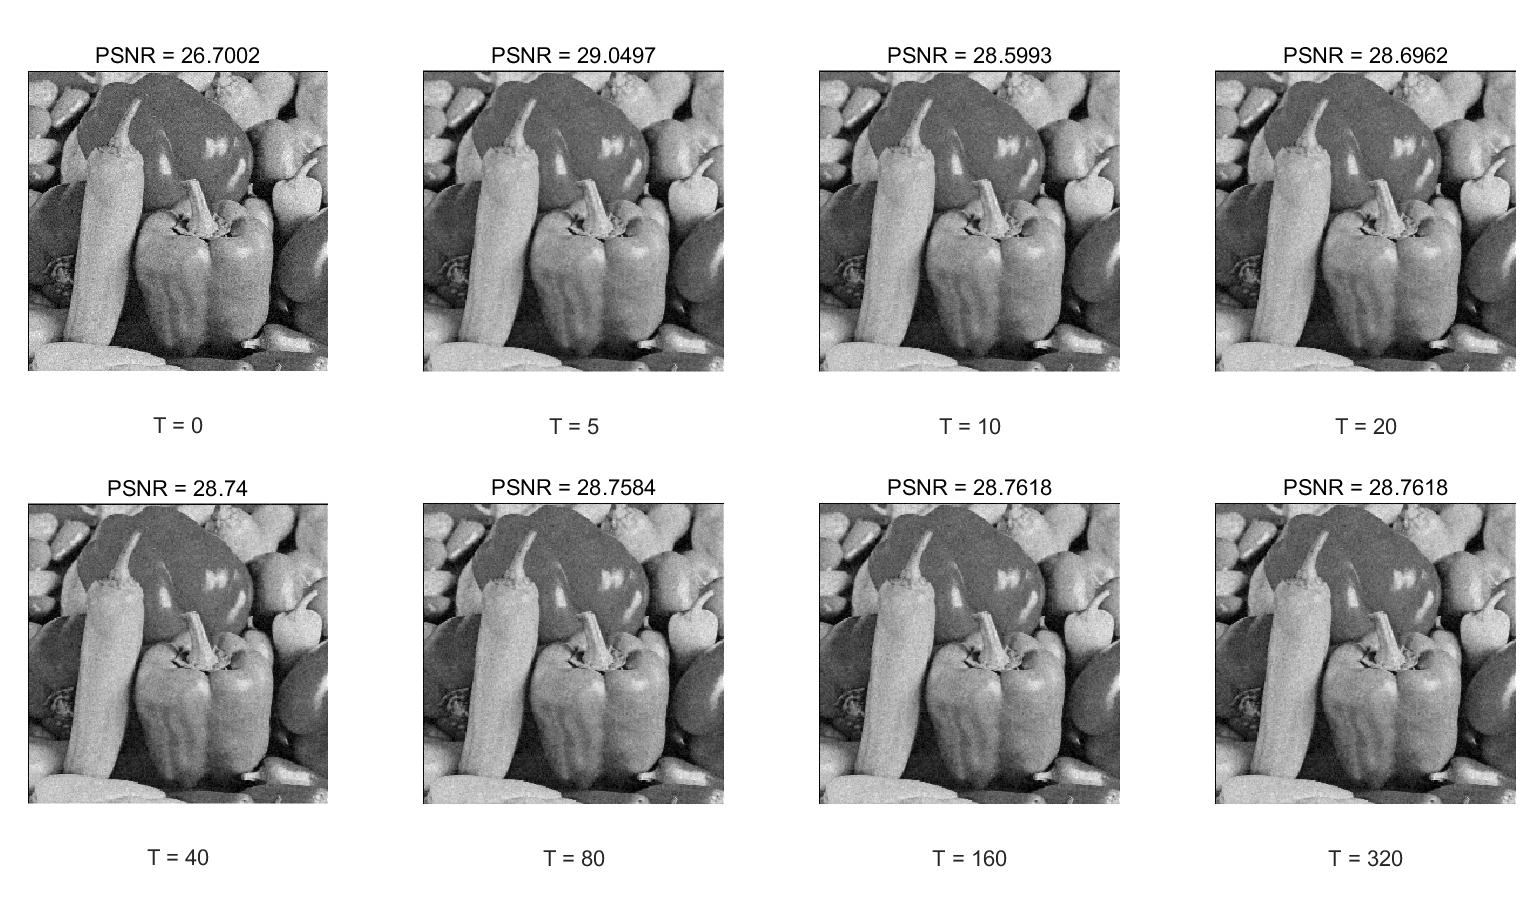
\includegraphics[scale=.38]{3.png}
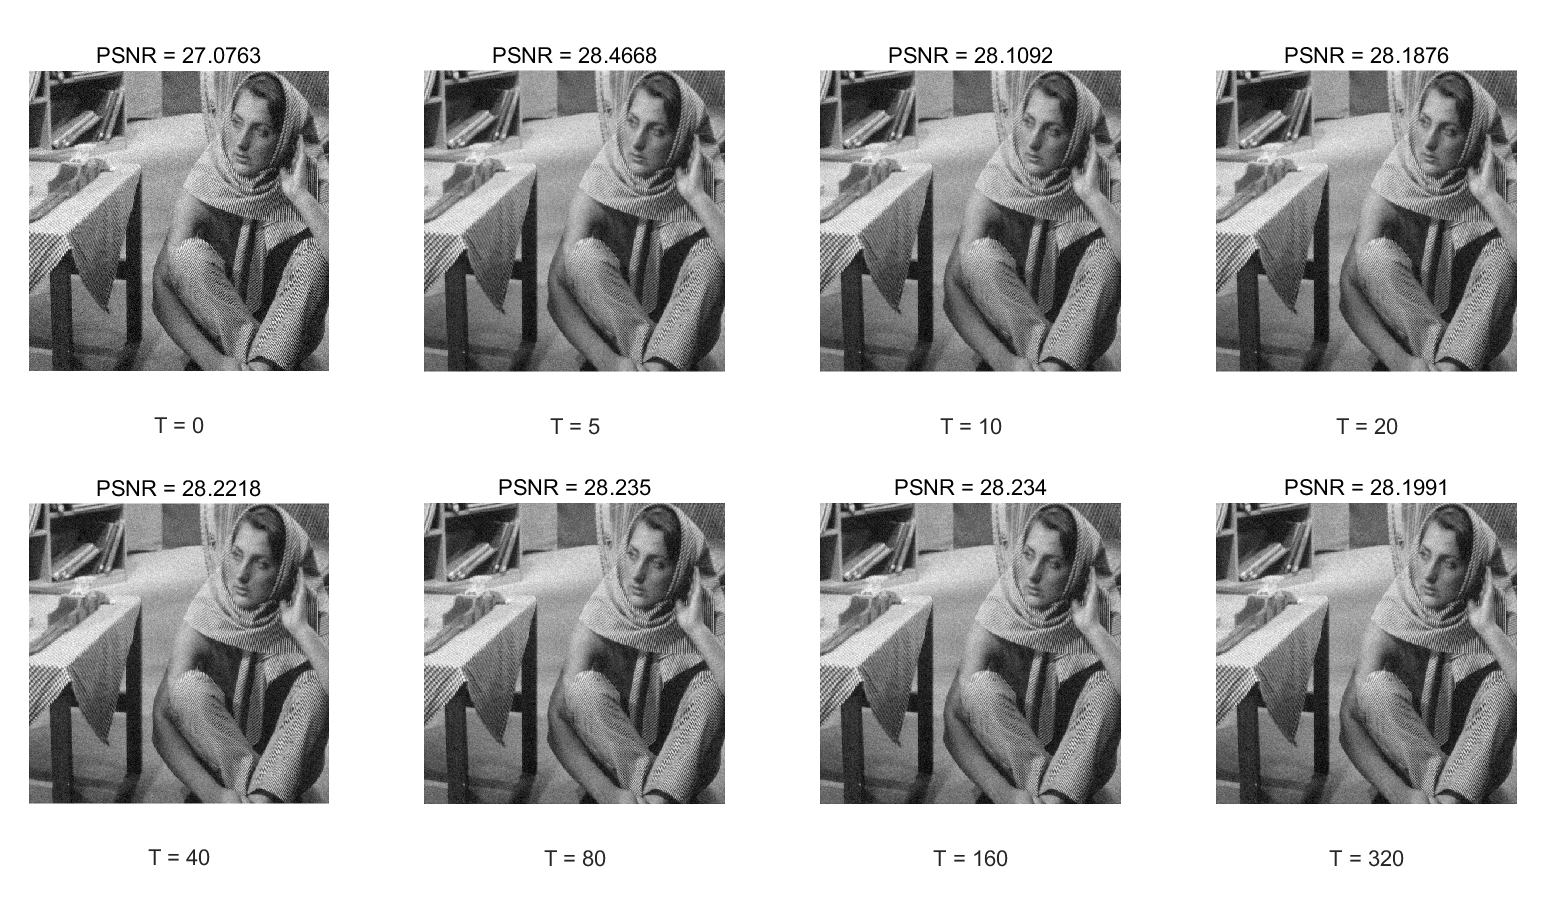
\includegraphics[scale=.38]{4.png}
\end{center}
\caption{Long time behaviour of Perona--Malik algorithm.}
\end{figure}

\section{Shock Filter}

\subsection{Algorithm}
Recall the shock filters in 2D
$$\frac{\partial v}{\partial t} = -|\nabla|F(L(v)),$$
the classical one for function:$L(v) = \triangle v$. 
As for a better choice, we claim:$L(v) = \frac{1}{{|\nabla u|}^2}(u_x^2 u_{xx}+u_x u_y u_{x,y} + u_y^2 u_{yy})$. 
Then we may write our model as
$$u^{n+1} = u^n  - \Delta t \sqrt{(\delta_x u^n)^2 + (\delta_y u^n)^2}F_{i,j}(L(u^n))$$
The typical choice of $F$ may be the sign function. $$F(u) = 0 \quad if \,\, u =0;\quad else \,\, u/|u|.$$

However, when the evolving time get longer, the result will be highly oscillating. To overcome this dilemma, we introduce two strategies:
\begin{enumerate}
\item Approximate L using central differencing.
\item Approximating the term $|\nabla v|$ using minmod operator
\begin{equation}
minmod(a,b) = \left\{ \begin{array}{cc} sign(a)\min (|a|, |b|) & if >0 \\0 & otherwise.\end{array}\right.
\end{equation}
And modify our function as:
$$u^{n+1} = u^n - \Delta t~\sqrt{(minmod(\delta_x^+u,\delta_x^-u)^2 + (minmod(\delta_y^+u,\delta_y^-u)^2}F(L(u)).$$
\end{enumerate}
In this report, we adopt the second modification.

\begin{algorithm}
\caption{$u = shock\_filter(f,T,\Delta t, F, L)$} 
\begin{algorithmic}[1]
\STATE $u = f$
\FOR{$i =1:T$}
\FOR{each direction $dir$}
\STATE compute the derivative $u_{dir}$
\ENDFOR
\STATE Compute $w = L(u)$.
\STATE Compute $y = F(w)$.
\STATE Compute $z = \sqrt{(minmod(\delta_x^+u,\delta_x^-u)^2 + (minmod(\delta_y^+u,\delta_y^-u)^2}$
\STATE $u^{n+1} = u^n -\Delta t ~ yz$
\ENDFOR
\end{algorithmic}
\end{algorithm}

\subsection{Numerical Result}
In this section we show the power of Rudin and Osher shock filter. We use two images downloaded from the Internet: `Camel' and the capital  `A`. We choose $\delta t = 0.05$

\begin{figure}[H]
\begin{center}
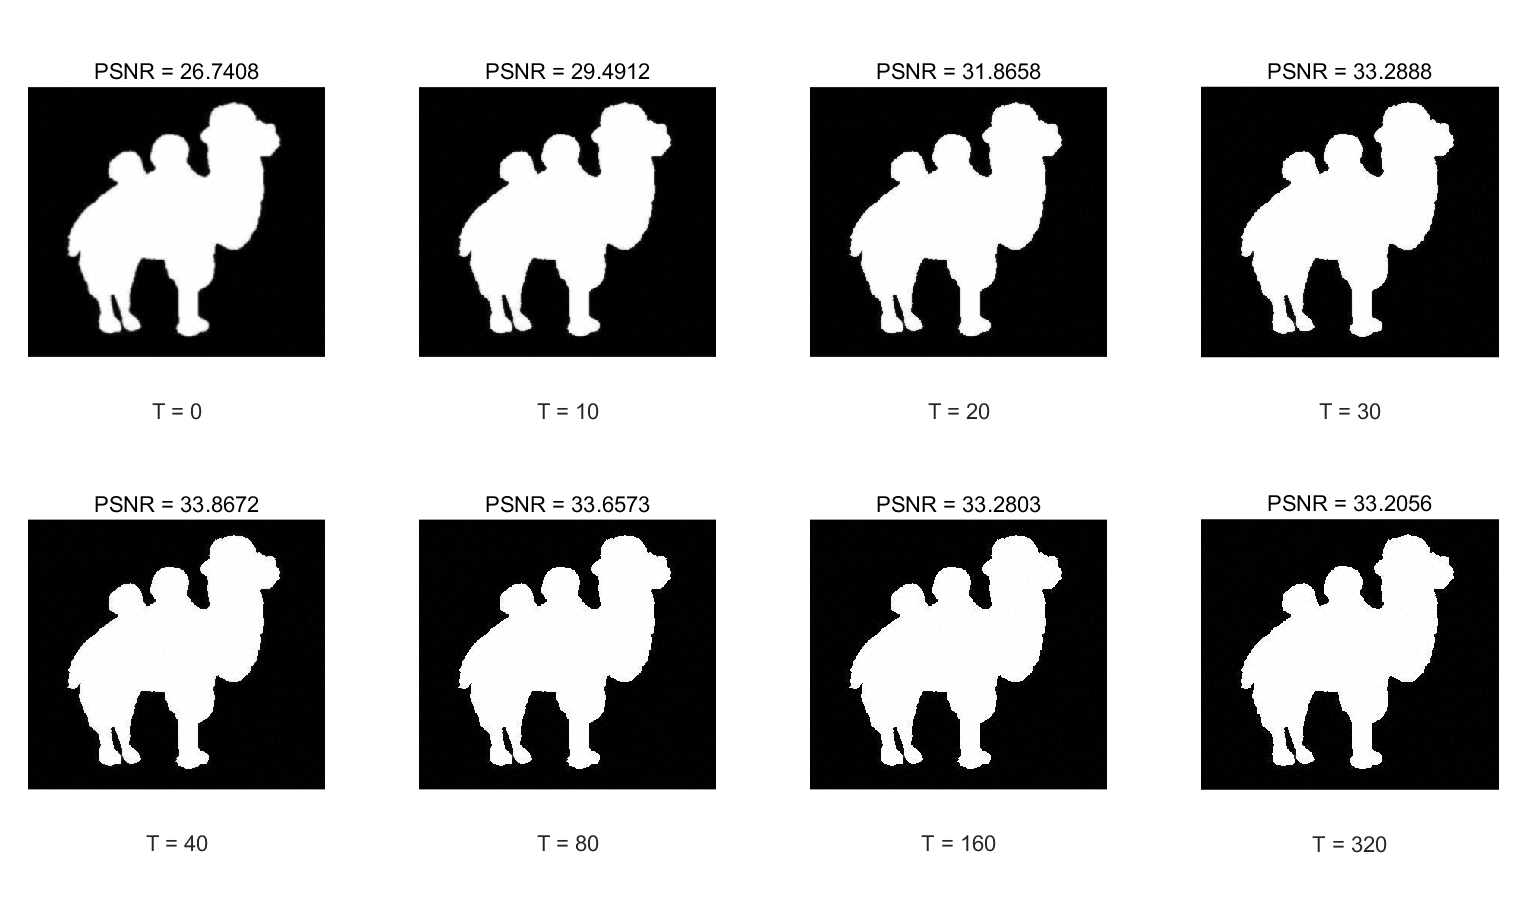
\includegraphics[scale=.31]{5.png}
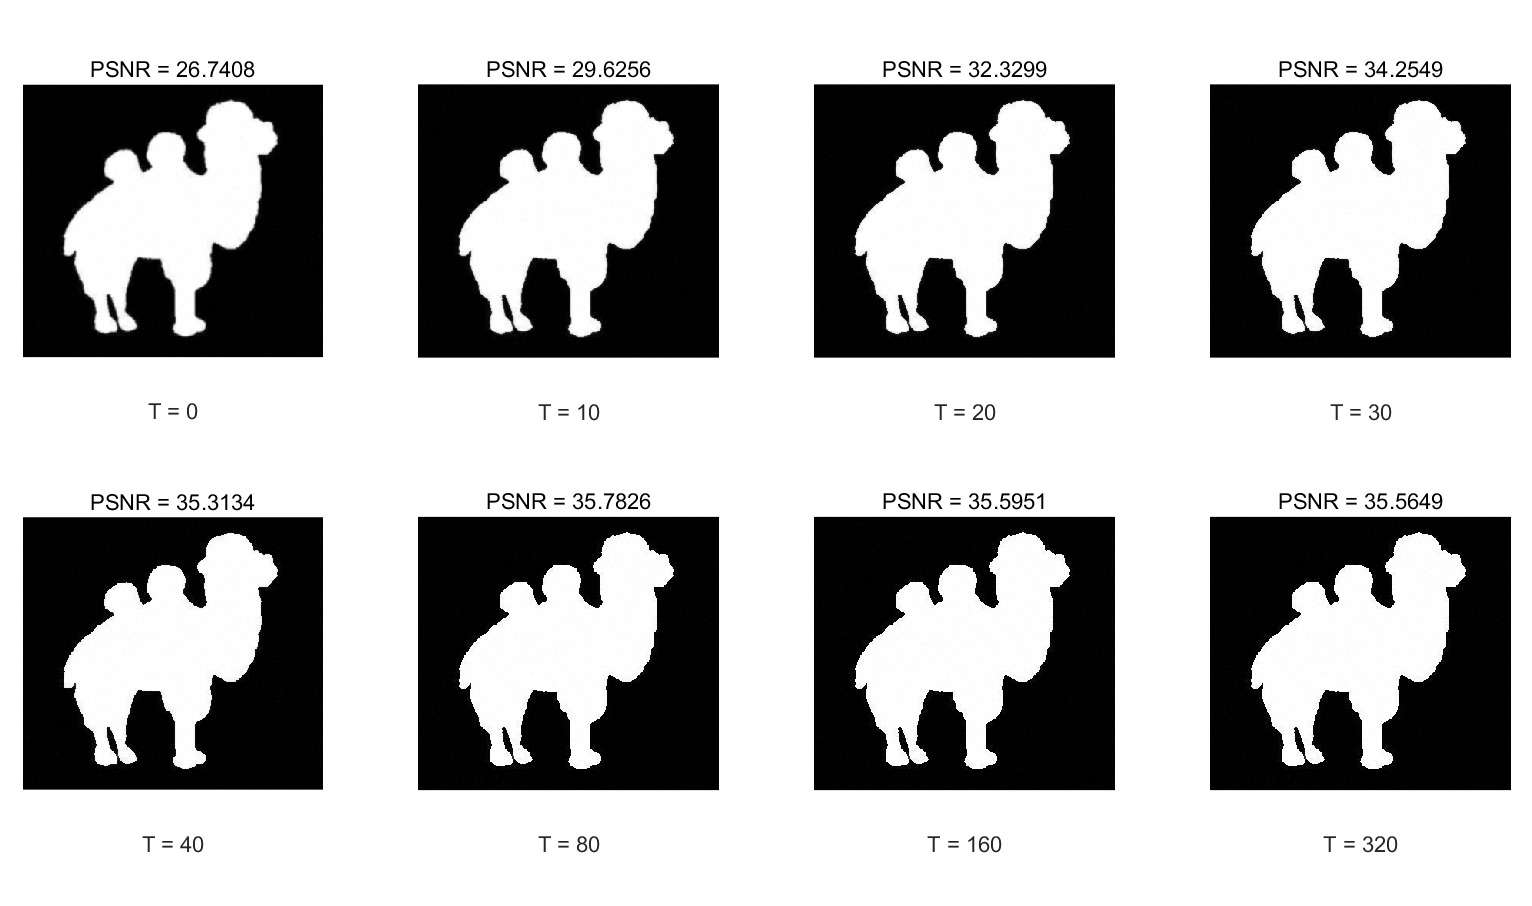
\includegraphics[scale=.31]{6.png}
\end{center}
\caption{We use the minmod to control the oscillation and it works well. Here the blur kernel = `fspecial('gaussian', [15,15],1)' with noise sigma = 0.01. The above one uses Laplacian as function L, and the other uses the better choice. We can see that the second choice of L bring better results, and the shock filter is somehow stable in the long time behaviour.}
\end{figure}

The next question is: what will the shock filter perform when the different level of noise is chosen. We fix $\Delta t$ as 0.05 and $T$ as 40, and the noise sigma = 0.01 0.02 0.05 0.1. The right picture is blured $f$, while the left one is enhanced $u$. This shows that when the noise level get higher, the result will be more oscillating.

\begin{figure}[H]
\begin{center}
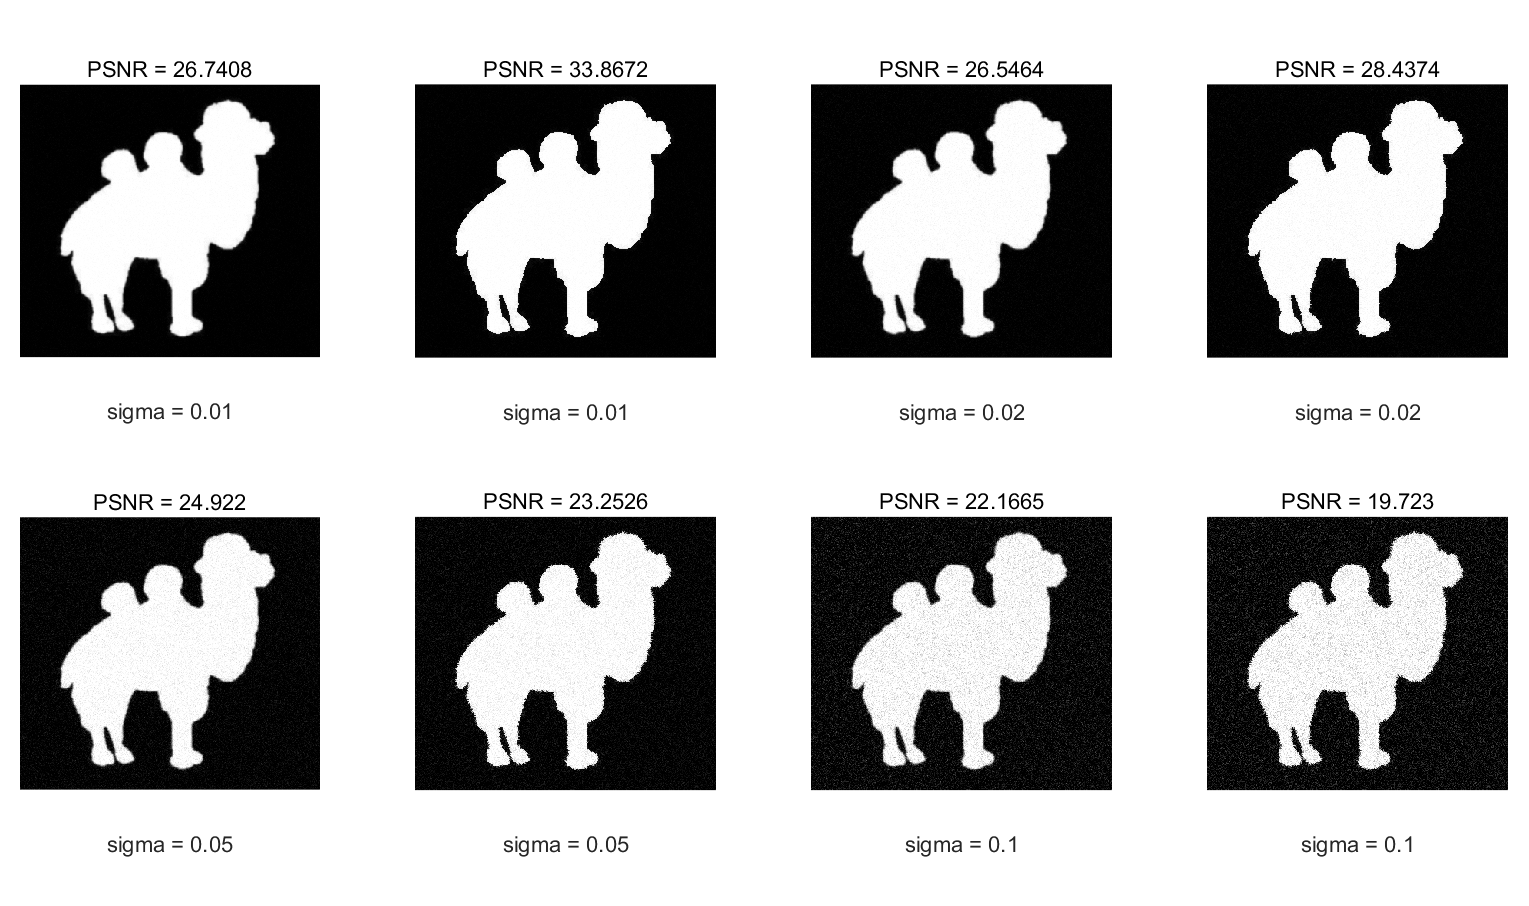
\includegraphics[scale=.36]{7.png}
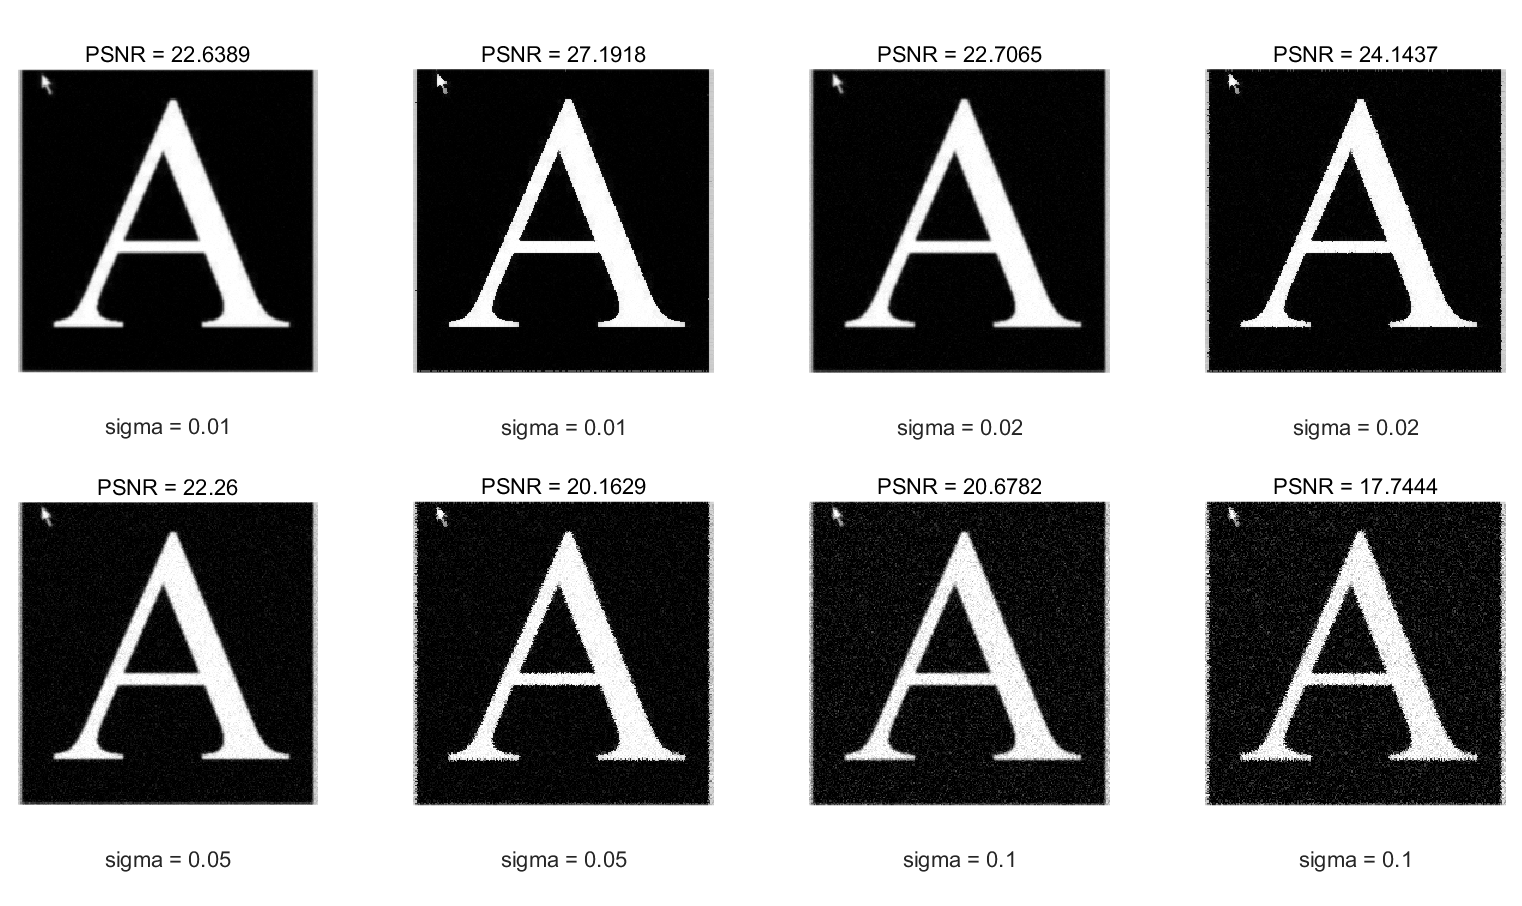
\includegraphics[scale=.36]{8.png}
\end{center}
\end{figure}

At last, we will discuss the performance of shock filter on natural image.

\begin{figure}[H]
\begin{center}
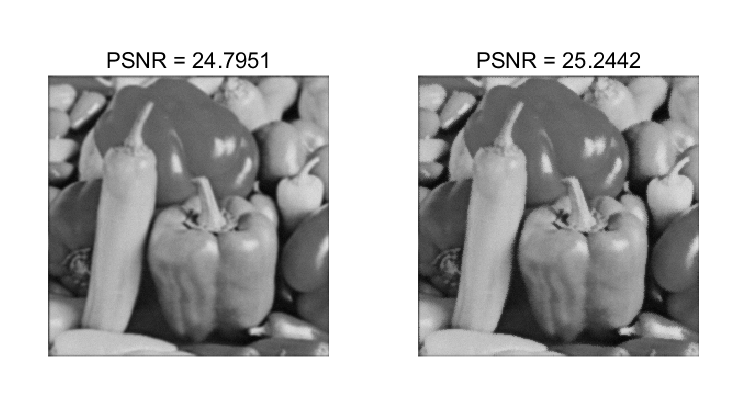
\includegraphics[scale=.7]{9.png}
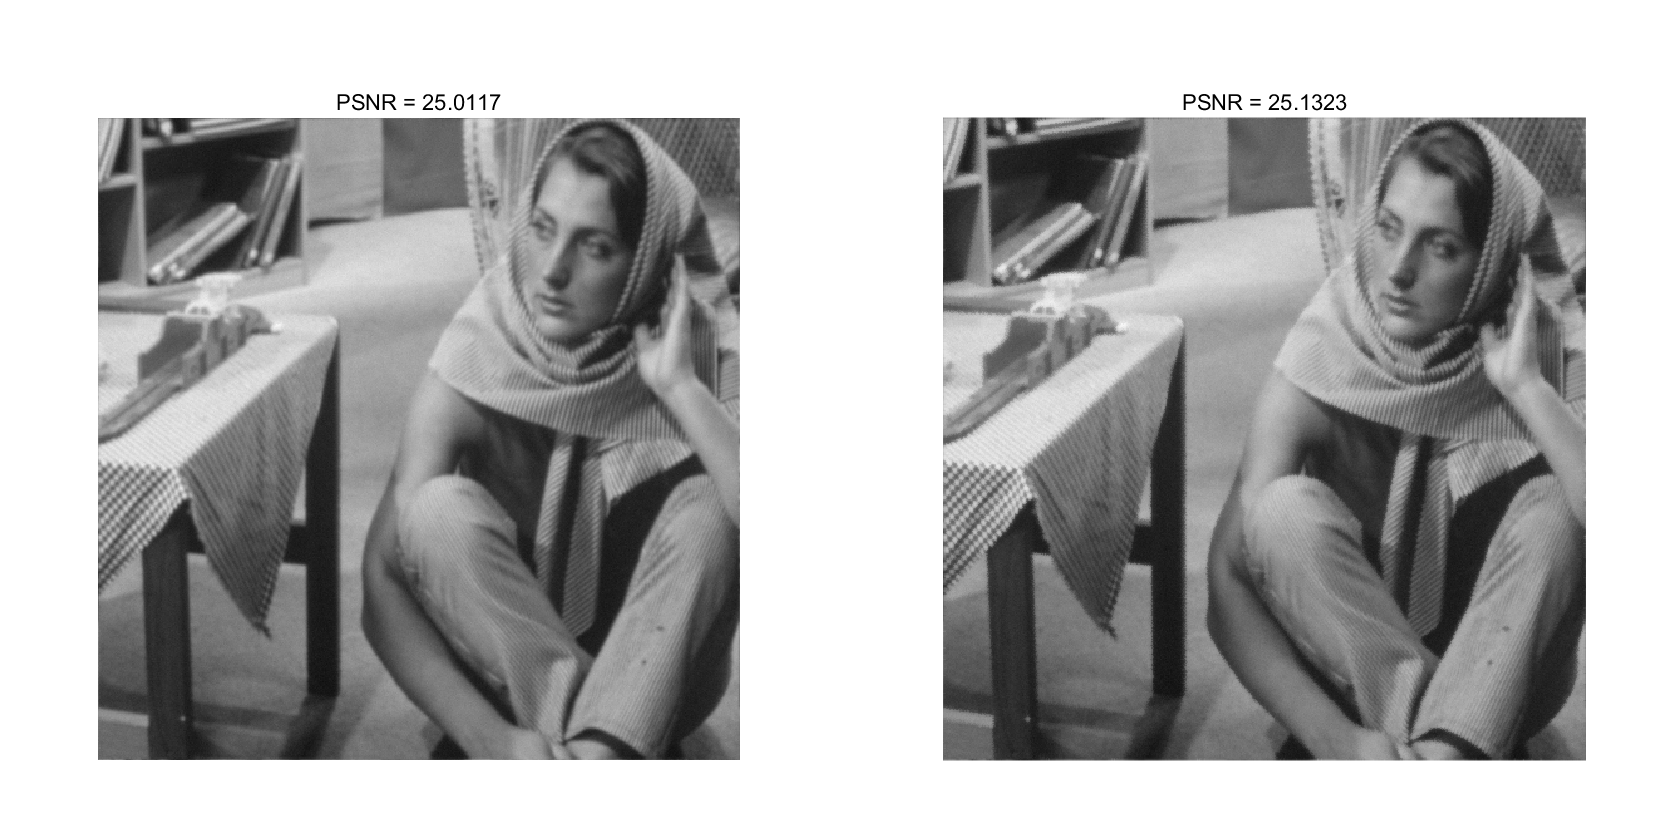
\includegraphics[scale=.3]{10.png}
\end{center}
\caption{The performance of the shock filter on natural image: Here the added noise sigma is 0.01. The blur kernel is `fspecial('gaussian', [15,15],1)'. Notice the algorithm could hardly enhance the edge entirely and the result is somehow oscillating.}
\end{figure}

\end{document}